\newpage
\section{Teachers}
First of all, if you haven't done it yet, you have to sign up inserting your name, surname, mail address, fiscal code, the unique code that had been given to you by the university personell and (optionally) a profile image.
After the login you will notice that a black bar has appeared near the top of the screen. 

\subsection{Exams List}
The black bar contains on its left the voice \textbf{Exams list}, if you click on that voice, you will be redirected to a page (similar to the one in Figure~\ref{fig:professorChooseExam}) that asks you to choose a class to which you had been assigned.
\begin{figure}[H]
	\centering
	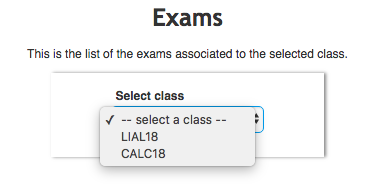
\includegraphics[width=0.65\textwidth]{img/professorChooseExam.png}
	\caption{Choiche of a class}
	\label{fig:professorChooseExam}
\end{figure}

After that, the page will be updated with a list of all the exams of your classes (similar to the one in Figure~\ref{fig:professorExamsList}).
\begin{figure}[H]
\centering
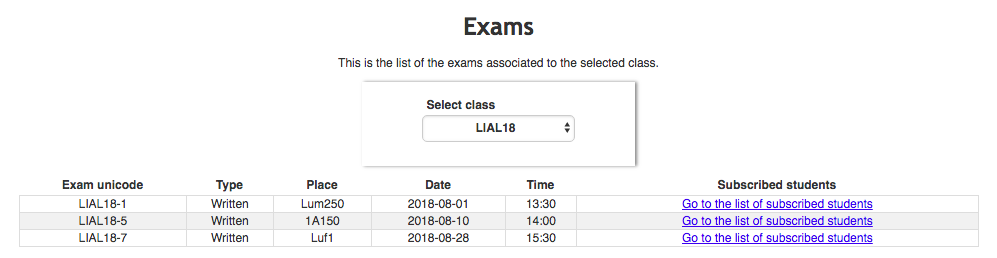
\includegraphics[width=1.0\textwidth]{img/professorExamsList.png}
\caption{List of the exams of a class}
\label{fig:professorExamsList}
\end{figure}

If you click on the link \textbf{Go to the list of subscribed students}, you will be redirected to a page that contains all the exams related to the selected course (as in Figure~\ref{fig:professorExamsMarks}).
\begin{figure}[H]
	\centering
	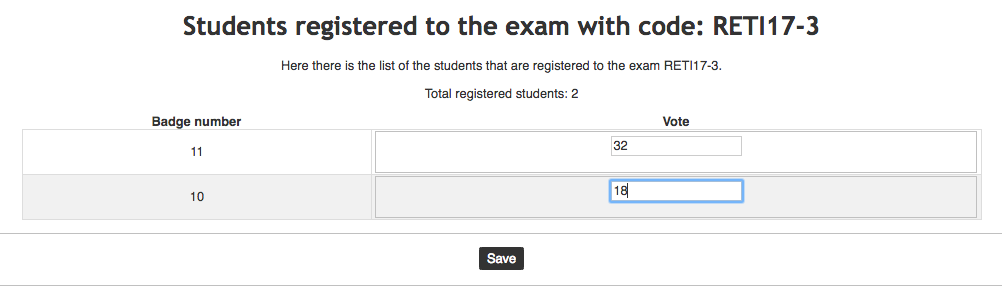
\includegraphics[width=1.0\textwidth]{img/professorExamsMarks.png}
	\caption{Marks given by the professor to his/her students}
	\label{fig:professorExamsMarks}
\end{figure}

You can give a mark to every student that is registered to the exam. The mark must be a number in the range \emph{0} - \emph{32}. To save the marks click on the button \textbf{Save}